\section{The Real Line and Coordinate Plane. Pythagoras}
\begin{introduction}
  \item The real line
  \item Inequalities
  \item Absolute values
  \item Intervals
  \item The coordinate plane
  \item The distance formula
  \item The midpoint formula
  \item Note on Pythagoras
\end{introduction}
\begin{questions}
  \item Among the words ``integer'', ``rational'', and ``irrational'', state the ones that apply to
  \begin{tasks}(4)
    \task \(-\frac{2}{3}\);
    \task \(0\);
    \task \(\frac{45}{9}\);
    \task \(0.75\);
    \task \(-\sqrt{49}\);
    \task \(\frac{1}{\pi}\);
    \task \(9.000...\);
    \task \(3^{1/2}\);
    \task \(-\frac{20}{7}\);
    \task \(\frac{94}{7}\).
  \end{tasks}

  \begin{note}
    \begin{itemize}
      \item \(\frac{45}{9} = 5\)
      \item \(-\sqrt{49} = -7\)
      \item \(9.000... = 9\)
    \end{itemize}
  \end{note}

  \begin{solution}
    \begin{itemize}
      \item Integer: \(0\), \(\frac{45}{9}\), \(-\sqrt{49}\), \(9.000...\);
      \item Rational: \(0\), \(\frac{45}{9}\), \(-\sqrt{49}\), \(9.000...\), \(-\frac{2}{3}\), \(0.75\), \(-\frac{20}{7}\), \(\frac{94}{7}\);
      \item Irrational: \(\frac{1}{\pi}\), \(3^{1/2}\).
    \end{itemize}
  \end{solution}

  \item Every integer is either even or odd. The even integers are those that are divisible by $2$, so $n$ is even if and only if it has the form $n=2k$ for some integer $k$. The odd integers are those that have the form $n=2k + 1$ for some integer $k$.
  \begin{tasks}
    \task If $n$ is even, prove that $n^2$ is also even.
    \task If $n$ is odd, prove that $n^2$ is also odd.
  \end{tasks}

  \begin{proof}
    \begin{tasks}
      \task Let $n$ be an even integer. By definition, there exist an integer $k$ such that $n=2k$.

      Consider $n^2$:

      $n^2=(2k)^2=4k^2=2(2k^2)$

      Since $2k^2$ is an integer, $n^2$ can be expressed in the form of $2m$ for integer $m=2k^2$, which implies that $n^2$ is even.

      Therefore, if $n$ is even, then $n^2$ is also even.
      \task Let $n$ be an odd integer. By definition, there exist an integer $k$ such that $n=2k+1$.

      Consider $n^2$:

      $n^2=(2k+1)^2 = 4k^2+4k+1=2(2k^2+2k) + 1$

      Since $2k^2+2k$ is an integer, $n^2$ can be expressed in the form of $n = 2m+1$ for integer $m=2k^2+2k$, which implies that $n^2$ is odd.

      Therefore, if $n$ is odd, then $n^2$ is also odd.
    \end{tasks}
  \end{proof}

  In Problems 3-12, rewrite the given expression without using the absolute value symbol.
  \begin{solution}
    \item $ \left| 7 - 18 \right| = 11 $.
    \item $ \left| 7 \right| - \left| - 18 \right| = -11 $.
    \item $ \left| \pi - 3\right| = \pi - 3 $.
    \item $ \left| 3 - \pi \right| = \pi - 3 $.
    \item $ \left| x - 5 \right| = 5 - x $ if $ x < 5 $.
    \item $ \left| x - 5 \right| = x - 5 $ if $ x > 5 $.
    \item $ \left| x^2 + 10 \right| = x^2 + 10$.
    \item $ \left| -11 \right| - \left| -10 \right| = 1 $.
    \item $ \left| 1 - 3x^2 \right| = 3x^2 - 1 $ if $ x \geq 1 $.
    \item $ \left| \sqrt{10} - 10 \right| = 10 - \sqrt{10} $.
  \end{solution}

  \item Solve the following inequalities:
  \begin{tasks}(3)
    \task $ x(x - 1) > 0 $;
    \task $ (x - 1)(x + 2) < 0 $;
    \task $ x^2 + 4x - 21 > 0 $;
    \task $ 2x^2 + x < 3 $;
    \task $ 4x^2 + 10x - 6 < 0 $;
    \task $ x^2 + 2x + 4 > 0 $;
  \end{tasks}

  \begin{note}

    \begin{multicols}{2}
      \begin{tikzpicture}
        % Define the center and axis lengths of the hyperbola
        \def\a{2}

        % Draw the x axis
        \draw[->] (-3,0) -- (3,0) node[right] {$x$};

        % Draw the parabola
        \draw[domain=-2:2,smooth,variable=\x,blue] plot ({\x},{(\x)^2 - \a});

        % Draw the vertices
        \filldraw[blue] ({sqrt(\a)},0) circle (1pt) node[below right] {root};
        \filldraw[blue] ({-sqrt(\a)},0) circle (1pt) node[below left] {root};

        % Write text at a specific position
        \node[right] at (2,1) {$+$};
        \node[left] at (-2,1) {$+$};
        \node[above] at (0,-1) {$-$};

      \end{tikzpicture}
      \columnbreak

      Quick tips for quadratic functions:
      \begin{enumerate}
        \item Draw the $x$-axis and plot the function.
        \item Mark the points where it intersects the $x$-axis as roots.
        \item The function is positive when it lies above the axis and negative when it lies below.
        \item If the quadratic term's negative, flip the graph!
      \end{enumerate}
    \end{multicols}
  \end{note}

  \begin{solution}
    \begin{tasks}
      \task $ x(x - 1) > 0 $;
      {
      \begin{note}
        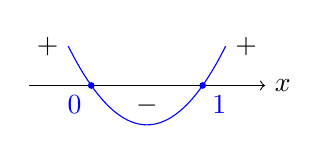
\begin{tikzpicture}
          \def\a{0.5}
          \draw[->] (-1.5,0) -- (1.5,0) node[right] {$x$};
          \draw[domain=-1:1,smooth,variable=\x,blue] plot ({\x},{(\x)^2 - \a});
          \filldraw[blue] ({-sqrt(\a)},0) circle (1pt) node[below left] {$0$};
          \filldraw[blue] ({sqrt(\a)},0) circle (1pt) node[below right] {$1$};
          \node[right] at (1,0.5) {$+$};
          \node[left] at (-1,0.5) {$+$};
          \node[above] at (0,-0.5) {$-$};
        \end{tikzpicture}
      \end{note}
      $x<0$ or $x>1$
      }
      \task $ (x - 1)(x + 2) < 0 $;
      {
      \begin{note}
        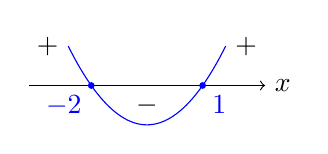
\begin{tikzpicture}
          \def\a{0.5}
          \draw[->] (-1.5,0) -- (1.5,0) node[right] {$x$};
          \draw[domain=-1:1,smooth,variable=\x,blue] plot ({\x},{(\x)^2 - \a});
          \filldraw[blue] ({-sqrt(\a)},0) circle (1pt) node[below left] {$-2$};
          \filldraw[blue] ({sqrt(\a)},0) circle (1pt) node[below right] {$1$};
          \node[right] at (1,0.5) {$+$};
          \node[left] at (-1,0.5) {$+$};
          \node[above] at (0,-0.5) {$-$};
        \end{tikzpicture}
      \end{note}
      $-2<x<1$
      }
      \task $ x^2 + 4x - 21 > 0 $;
      {
      \begin{note}
        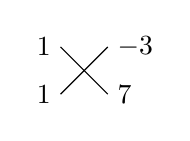
\begin{tikzpicture}
          \def\a{0.3}
          \draw[-] (-\a,\a) node[left] {$1$} -- (\a,-\a) node[right] {$7$};
          \draw[-] (-\a,-\a) node[left] {$1$} -- (\a,\a) node[right] {$-3$};
        \end{tikzpicture}

        $ (x+7)(x-3) > 0 $

        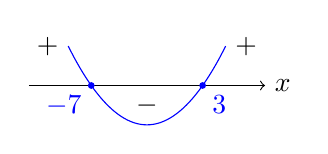
\begin{tikzpicture}
          \def\a{0.5}
          \draw[->] (-1.5,0) -- (1.5,0) node[right] {$x$};
          \draw[domain=-1:1,smooth,variable=\x,blue] plot ({\x},{(\x)^2 - \a});
          \filldraw[blue] ({-sqrt(\a)},0) circle (1pt) node[below left] {$-7$};
          \filldraw[blue] ({sqrt(\a)},0) circle (1pt) node[below right] {$3$};
          \node[right] at (1,0.5) {$+$};
          \node[left] at (-1,0.5) {$+$};
          \node[above] at (0,-0.5) {$-$};
        \end{tikzpicture}
      \end{note}
      $x<-7$ or $x>3$
      }
      \task $ 2x^2 + x < 3 $;
      {
      \begin{note}
        $2x^2 + x -3 < 0$

        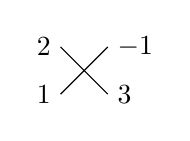
\begin{tikzpicture}
          \def\a{0.3}
          \draw[-] (-\a,\a) node[left] {$2$} -- (\a,-\a) node[right] {$3$};
          \draw[-] (-\a,-\a) node[left] {$1$} -- (\a,\a) node[right] {$-1$};
        \end{tikzpicture}

        $ (2x+3)(x-1) < 0 $

        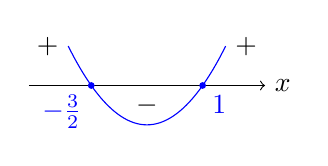
\begin{tikzpicture}
          \def\a{0.5}
          \draw[->] (-1.5,0) -- (1.5,0) node[right] {$x$};
          \draw[domain=-1:1,smooth,variable=\x,blue] plot ({\x},{(\x)^2 - \a});
          \filldraw[blue] ({-sqrt(\a)},0) circle (1pt) node[below left] {$-\frac{3}{2}$};
          \filldraw[blue] ({sqrt(\a)},0) circle (1pt) node[below right] {$1$};
          \node[right] at (1,0.5) {$+$};
          \node[left] at (-1,0.5) {$+$};
          \node[above] at (0,-0.5) {$-$};
        \end{tikzpicture}
      \end{note}
      $-\frac{3}{2} < x < 1$
      }
      \task $ 4x^2 + 10x - 6 < 0 $;
      {
      \begin{note}
        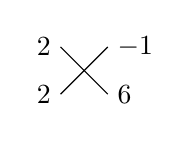
\begin{tikzpicture}
          \def\a{0.3}
          \draw[-] (-\a,\a) node[left] {$2$} -- (\a,-\a) node[right] {$6$};
          \draw[-] (-\a,-\a) node[left] {$2$} -- (\a,\a) node[right] {$-1$};
        \end{tikzpicture}

        $ (2x+6)(2x-1) < 0 $

        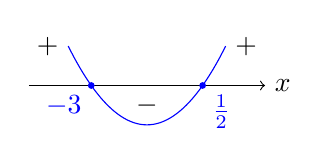
\begin{tikzpicture} % quadratic
          \def\a{0.5}
          \draw[->] (-1.5,0) -- (1.5,0) node[right] {$x$};
          \draw[domain=-1:1,smooth,variable=\x,blue] plot ({\x},{(\x)^2 - \a});
          \filldraw[blue] ({-sqrt(\a)},0) circle (1pt) node[below left] {$-3$};
          \filldraw[blue] ({sqrt(\a)},0) circle (1pt) node[below right] {$\frac{1}{2}$};
          \node[right] at (1,0.5) {$+$};
          \node[left] at (-1,0.5) {$+$};
          \node[above] at (0,-0.5) {$-$};
        \end{tikzpicture}
      \end{note}
      $-3<x<\frac{1}{2}$
      }
      \task $ x^2 + 2x + 4 > 0 $;
      {
      \begin{note}
        $\Delta = 2^2-4\times4 = -12 < 0$

        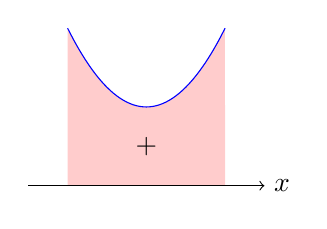
\begin{tikzpicture} % quadratic 1 root
          \fill[red!20](-1,0) -- plot[domain=-1:1, samples=200] (\x, {(\x)^2 + 1}) -- (1,0) -- cycle;
          \draw[domain=-1:1,smooth,variable=\x,blue] plot ({\x},{(\x)^2 + 1});
          \draw[->] (-1.5,0) -- (1.5,0) node[right] {$x$};

          \node at (0,0.5) {$+$};
        \end{tikzpicture}
      \end{note}
      all x
      }

    \end{tasks}

  \end{solution}
  \item Recall that $\sqrt{a}$ is a real number if and only if $a \geq 0$, and find the values of $x$ for which each of the following is a real number:
  \begin{tasks}
    \task $\sqrt{4-x^2}$;

    \begin{solution}
      $\sqrt{4-x^2}$ is rational means $4-x^2 \geq 0$, then $-2 \leq x \leq 2$.
    \end{solution}

    \task $\sqrt{x^2-9}$;

    \begin{solution}
      $\sqrt{x^2-9}$ is rational means $x^2-9 \geq 0$, then $x \leq -3$ or $x \geq 3$.
    \end{solution}

    \task \(\frac{1}{\sqrt{4-3x}}\);

    \begin{solution}
      \(\frac{1}{\sqrt{4-3x}}\) is rational means $4-3x>0$, then \(x < \frac{4}{3}\).
    \end{solution}

    \task \(\frac{1}{\sqrt{x^2-x-12}}\);

    \begin{solution}
      \(\frac{1}{\sqrt{x^2-x-12}}\) is rational means $x^2-x-12>0$, then $x<-3$ or $x>4$.
    \end{solution}

  \end{tasks}

  \item Find the values of $x$ for which each of the following is positive:
  \begin{tasks}
    \task \(\frac{x}{x^2+4}\);

    \begin{solution}
      The denominator $x^2+4$ is always positive. Therefore, for the fraction to be positive, the numerator $x$ must also be positive. Hence, the solution is $x>0$.
    \end{solution}

    \task \(\frac{x}{x^2-4}\);

    \begin{solution}
      \begin{note}
        \begin{tikzpicture} % cubic
          \draw[->] (-3,0) -- (3,0) node[right] {$x$};
          \draw[blue, domain=-3*pi/4:3*pi/4, samples=200] plot (\x, {-2*sin(deg(2*\x))});
          \draw[blue] ({-pi/2},0) circle (1pt) node[below right] {$-2$};
          \draw[blue] (0,0) circle (1pt) node[below left] {$0$};
          \draw[blue] ({pi/2},0) circle (1pt) node[below right] {$2$};
          \node[right] at ({3*pi/4},1) {$+$};
          \node at ({pi/4},-1) {$-$};
          \node at ({-pi/4},1) {$+$};
          \node[left] at ({-3*pi/4},-1) {$-$};
        \end{tikzpicture}

        Sketches can be used to determine the regions of $x$ quickly:
        \begin{enumerate}
          \item Draw a sketch ensuring it intersects the $x$-axis the same number of times as the number of terms containing $x$ after factorization.
          \item Sketch from right to left. If the highest degree of $x$ is positive, start above the $x$-axis, if it's negative, start below the $x$-axis.
          \item Mark the points where it intersects the $x$-axis as roots.
          \item The function is positive when it lies above the $x$-axis and negative when it lies below.
        \end{enumerate}
      \end{note}

      $-2<x<0$ or $x>2$.
    \end{solution}

    \task \(\frac{x+1}{x-3}\);

    \begin{solution}
      \begin{note}
        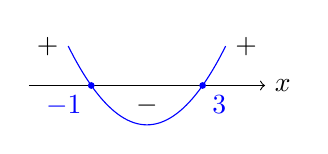
\begin{tikzpicture} % quadratic
          \def\a{0.5}
          \draw[->] (-1.5,0) -- (1.5,0) node[right] {$x$};
          \draw[domain=-1:1,smooth,variable=\x,blue] plot ({\x},{(\x)^2 - \a});
          \filldraw[blue] ({-sqrt(\a)},0) circle (1pt) node[below left] {$-1$};
          \filldraw[blue] ({sqrt(\a)},0) circle (1pt) node[below right] {$3$};
          \node[right] at (1,0.5) {$+$};
          \node[left] at (-1,0.5) {$+$};
          \node[above] at (0,-0.5) {$-$};
        \end{tikzpicture}
      \end{note}

      $x<-1$ or $x>3$.
    \end{solution}

    \task \(\frac{x^2-1}{x^2-3x}\);

    \begin{solution}
      \begin{note}
        First, factorize the expression and get \(\frac{(x+1)(x-1)}{x(x-3)}>0\)

        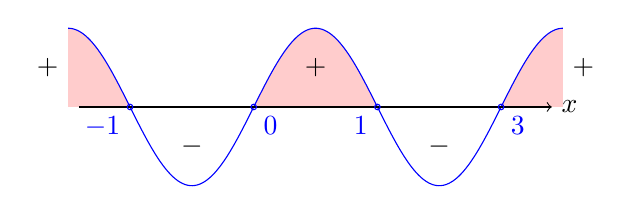
\begin{tikzpicture} % cubic
          \fill[red!20](-pi,0) -- plot[domain=-pi:pi, samples=200] (\x, {cos(deg(2*\x)) > 0 ? cos(deg(2*\x)) : 0}) -- (pi,0) -- cycle;
          \draw[blue, domain=-pi:pi, samples=200] plot (\x, {cos(deg(2*\x))});
          \draw[->] (-3,0) -- (3,0) node[right] {$x$};

          \draw[blue] ({-3*pi/4},0) circle (1pt) node[below left] {$-1$};
          \draw[blue] ({-pi/4},0) circle (1pt) node[below right] {$0$};
          \draw[blue] ({pi/4},0) circle (1pt) node[below left] {$1$};
          \draw[blue] ({3*pi/4},0) circle (1pt) node[below right] {$3$};
          \node[right] at ({pi},0.5) {$+$};
          \node at ({pi/2},-0.5) {$-$};
          \node at (0,0.5) {$+$};
          \node at ({-pi/2},-0.5) {$-$};
          \node[left] at ({-pi},+0.5) {$+$};
        \end{tikzpicture}

      \end{note}

      $x<-1$, $0<x<1$ or $x>3$.
    \end{solution}

  \end{tasks}
  \item State the values of $a$ for which the following inequalities are valid:
  \begin{tasks}(2)
    \task $a \leq a$;

    \begin{solution}
      All $a$.
    \end{solution}

    \task $a<a$;

    \begin{solution}
      None $a$.
    \end{solution}

  \end{tasks}
  \item If $a \leq b$ and $b \leq a$, what conclusion can be drawn about $a$ and $b$?

  \begin{solution}
    $a=b$.
  \end{solution}

  \item \begin{tasks}
    \task If $a<b$ is true, is it also necessarily true that $a \leq b$?

    \begin{solution}
      Yes.
    \end{solution}

    \task If $a \leq b$ is true, is it also necessarily true that $a<b$?

    \begin{solution}
      No. When $a=b$, $a \leq b$ is true but $a<b$ is false.
    \end{solution}

  \end{tasks}

  \item State whether each pair of points lies on a horizontal or a vertical line:
  \begin{tasks}(2)
    \task $(-2, -5)$, $(-2, -3)$;

    \begin{solution}
      Vertical.
    \end{solution}

    \task $(-2, -5)$, $(7, -5)$;

    \begin{solution}
      Horizontal.
    \end{solution}

    \task $(-3, 4)$, $(6, 4)$;

    \begin{solution}
      Horizontal.
    \end{solution}

    \task $(2, -11)$, $(2, 5)$;

    \begin{solution}
      Vertical.
    \end{solution}

    \task $(2, 2)$, $(-13, 2)$;

    \begin{solution}
      Horizontal.
    \end{solution}

    \task $(-7, -7)$, $(-7, 7)$;

    \begin{solution}
      Vertical.
    \end{solution}

    \task $(3, 5)$, $(3, -2)$;

    \begin{solution}
      Vertical.
    \end{solution}

    \task $(-1, -2)$, $(2, -2)$.

    \begin{solution}
      Horizontal.
    \end{solution}

  \end{tasks}

  \item Three vertices of a rectangle are $(-1, 2)$, $(3, -5)$, $(-1, -5)$. What is the fourth vertex?

  \begin{solution}
    \begin{note}
      \begin{tikzpicture} % rectangle
        \draw[->] (-3,0) -- (3,0) node[right] {$x$};
        \draw[->] (0,-3) -- (0,3) node[above] {$y$};
        \draw[blue] (-1/2, 2/2) -- (-1/2, -5/2);
        \draw[blue] (-1/2, -5/2) -- (3/2, -5/2);
        \draw[dashed, blue] (3/2, -5/2) -- (3/2, 2/2);
        \draw[dashed, blue] (3/2, 2/2) -- (-1/2, 2/2);
        \draw[dashed, red] (-1/2, 2/2) -- (3/2, -5/2);
        \draw[dashed, red] (-1/2, -5/2) -- (3/2, 2/2);
        \filldraw[blue] (-1/2, 2/2) circle (1pt) node[above left] {$(-1, 2)$};
        \filldraw[blue] (3/2, -5/2) circle (1pt) node[below right] {$(3, -5)$};
        \filldraw[blue] (-1/2, -5/2) circle (1pt) node[below left] {$(-1, -5)$};
        \draw[blue] (3/2, 2/2) circle (1pt) node[above right] {$(3, 2)$};
        \draw[red] (1/2, -3/4) circle (1pt) node[right] {$(1, -3/2)$};
      \end{tikzpicture}
    \end{note}

    As the sides of the rectangle are parallel to the x-axis or y-axis, We can easily find the fourth vertex is $(3, 2)$.

    Alternatively, we can calculate it using the midpoint formulas:

    Assuming the forth point is $P(x,y)$, the midpoints of the line segment connecting the first and second vertices, and the third and forth vertices, should be the same point. Thus, we have \(\frac{x-1}{2} = \frac{-1+3}{2} \) and \(\frac{y-5}{2} = \frac{2-5}{2}\). So $x=3$ and $y=2$.

  \end{solution}

  \item Find the distance between each pair of points: \label{sec_01_02:1}

  \begin{tasks}(2)
    \task $(1,2)$, $(6,7)$;
    \task $(2,5)$, $(-1,3)$;
    \task $(-7, 3)$, $(1, -2)$;
    \task $(a, b)$, $(b, a)$.
  \end{tasks}
  \begin{tasks}
    \task $(1,2)$, $(6,7)$;
    \begin{solution}
      $d=\sqrt{(6-1)^2+(7-2)^2}=5\sqrt{2}$
    \end{solution}
    \task $(2,5)$, $(-1,3)$;
    \begin{solution}
      $d=\sqrt{(2+1)^2+(5-3)^2}=\sqrt{13}$
    \end{solution}
    \task $(-7, 3)$, $(1, -2)$;
    \begin{solution}
      $d=\sqrt{(1+7)^2+(3+2)^2}=\sqrt{89}$
    \end{solution}
    \task $(a, b)$, $(b, a)$.
    \begin{solution}
      $d=\sqrt{(b-a)^2+(a-b)^2}=\left| b-a \right| \sqrt{2}$
    \end{solution}
  \end{tasks}

  \item In Problem \ref{sec_01_02:1} find the midpoint of the segment joining each pair of points.

  \begin{tasks}
    \task $(1,2)$, $(6,7)$;
    \begin{solution}
      \(x=\frac{6+1}{2} = \frac{7}{2}\), \(y=\frac{7+2}{2}=\frac{9}{2}\)
    \end{solution}
    \task $(2,5)$, $(-1,3)$;
    \begin{solution}
      \(x=\frac{2-1}{2}=\frac{1}{2}\), \(y=\frac{5+3}{2}=4\)
    \end{solution}
    \task $(-7, 3)$, $(1, -2)$;
    \begin{solution}
      \(x=\frac{-7+1}{2}=-3\), \(y=\frac{3-2}{2}=\frac{1}{2}\)
    \end{solution}
    \task $(a, b)$, $(b, a)$.
    \begin{solution}
      \(x=\frac{a+b}{2}\), \(y=\frac{a+b}{2}\)
    \end{solution}
  \end{tasks}

  \item Draw a sketch indicating the points (x, y) in the plane for which
  \begin{tasks}(2)
    \task $x<2$;
    \task $-1<y \leq 2$;
    \task $0 \leq x \leq 1$ and $0 \leq y \leq 1$;
    \task $x=-1$;
    \task $y=3$;
    \task $x=y$.
  \end{tasks}

  \begin{tasks}(2)
    \task $x<2$;
    \begin{solution}

      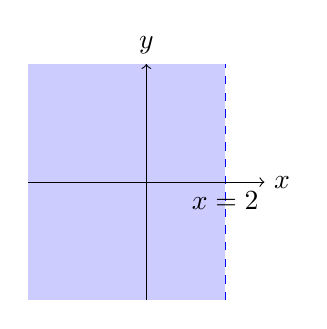
\begin{tikzpicture} % rectangle
        % Region where x < 2
        \fill[blue!20] (-1.5,1.5) -- (-1.5,-1.5) -- (1,-1.5) -- (1,1.5) -- cycle;
        \draw[blue, dashed] (1,-1.5) -- (1,1.5);
        \draw[->] (-1.5,0) -- (1.5,0) node[right] {$x$};
        \draw[->] (0,-1.5) -- (0,1.5) node[above] {$y$};
        \node[below] at (1,0) {$x = 2$};
      \end{tikzpicture}
    \end{solution}

    \task $-1<y \leq 2$;
    \begin{solution}

      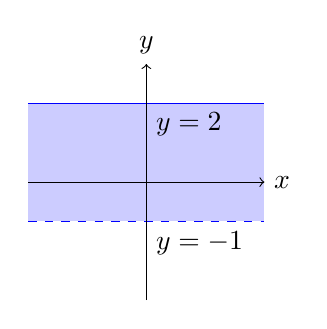
\begin{tikzpicture} % rectangle
        % Region where x < 2
        \fill[blue!20] (-1.5,1) -- (-1.5,-0.5) -- (1.5,-0.5) -- (1.5,1) -- cycle;
        \draw[blue, dashed] (-1.5,-0.5) -- (1.5,-0.5);
        \draw[blue] (-1.5,1) -- (1.5,1);
        \draw[->] (-1.5,0) -- (1.5,0) node[right] {$x$};
        \draw[->] (0,-1.5) -- (0,1.5) node[above] {$y$};
        \node[below right] at (0,1) {$y = 2$};
        \node[below right] at (0,-0.5) {$y = -1$};
      \end{tikzpicture}
    \end{solution}

    \task $0 \leq x \leq 1$ and $0 \leq y \leq 1$;
    \begin{solution}

      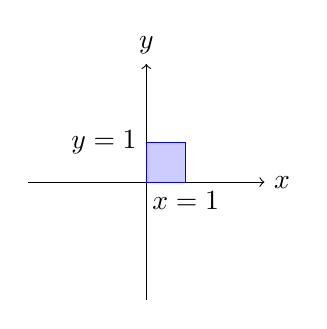
\begin{tikzpicture} % rectangle
        % Region where x < 2
        \fill[blue!20] (0,0) -- (0.5,0) -- (0.5,0.5) -- (0,0.5) -- cycle;
        \draw[->] (-1.5,0) -- (1.5,0) node[right] {$x$};
        \draw[->] (0,-1.5) -- (0,1.5) node[above] {$y$};
        \draw[blue] (0,0) -- (0.5,0);
        \draw[blue] (0.5,0) -- (0.5,0.5);
        \draw[blue] (0.5,0.5) -- (0,0.5);
        \draw[blue] (0,0.5) -- (0,0);
        \node[left] at (0,0.5) {$y = 1$};
        \node[below] at (0.5,0) {$x = 1$};
      \end{tikzpicture}
    \end{solution}

    \task $x=-1$;
    \begin{solution}

      \begin{tikzpicture} % rectangle
        \draw[->] (-1.5,0) -- (1.5,0) node[right] {$x$};
        \draw[->] (0,-1.5) -- (0,1.5) node[above] {$y$};
        \draw[blue] (-0.5,1.5) -- (-0.5,-1.5);
        \node[below] at (-0.6,0) {$x = -1$};
      \end{tikzpicture}
    \end{solution}

    \task $y=3$;
    \begin{solution}

      \begin{tikzpicture} % rectangle
        \draw[->] (-1.5,0) -- (1.5,0) node[right] {$x$};
        \draw[->] (0,-1.5) -- (0,1.5) node[above] {$y$};
        \draw[blue] (-1.5,1) -- (1.5,1);
        \node[below right] at (0,1) {$y = 3$};
      \end{tikzpicture}
    \end{solution}

    \task $x=y$.
    \begin{solution}

      \begin{tikzpicture} % rectangle
        \draw[->] (-1.5,0) -- (1.5,0) node[right] {$x$};
        \draw[->] (0,-1.5) -- (0,1.5) node[above] {$y$};
        \draw[blue] (-1,-1) -- (1,1);
        \node[below right] at (1,1) {$x = y$};
      \end{tikzpicture}
    \end{solution}
  \end{tasks}

  \item Use the distance formula to show that the points $(-2, 1)$, $(2,2)$, and $(10, 4)$ lie on a straight line.
  \begin{proof}
    Given points $P_1(-2, 1)$, $P_2(2,2)$ and $P_3(10,4)$.

    Using the distance formula, the distance between $P_1$ and $P_2$ is:

    $d_{12} = \sqrt{(2+2)^2+(2-1)^2}=\sqrt{17}$,

    The distance between $P_2$ and $P_3$ is:

    $d_{23} = \sqrt{(10-2)^2+(4-2)^2}=\sqrt{68}=2\sqrt{17}$,

    And the distance between $P_1$ and $P_3$ is:

    $d_{13} = \sqrt{(10+2)^2+(4-1)^2}=\sqrt{153}=3\sqrt{17}$.

    Now, we observe that $d_{13} = d_{12}+d_{23}$.

    This verifies that the points $(-2, 1)$, $(2,2)$, and $(10, 4)$ lie on a straight line.
  \end{proof}
\end{questions}